\documentclass{report}
\usepackage[utf8]{inputenc}

% Títulos automáticos en español
\usepackage[english]{babel}

% Soporte para buenas urls e hipervínculos entre secciones
\usepackage{hyperref}

% Citas y referencias en formato APA
% Si quiere las citas y referencias en IEEE comente esta línea
\usepackage{apacite}

% Imágenes y figuras
\usepackage{graphicx}

% Código fuente con números de línea
\usepackage{listings}
% Puede cambiar el lenguaje de código fuente
% https://www.overleaf.com/learn/latex/code_listing#Supported_languages
\lstset{
    language=C,
    basicstyle=\footnotesize,
    numbers=left,
    stepnumber=1,
    showstringspaces=false,
    tabsize=1,
    breaklines=true,
    breakatwhitespace=false,
}

\usepackage{tikz}
\usetikzlibrary{positioning, arrows.meta}

\def \unidad{Computer Engineering Department}
\def \programa{Computer Engineering}
\def \curso{IC5701 - Compilers \& Interpreters}
\def \subtitulo {Dr. Francisco J. Torres-Rojas}
\def \titulo{Deterministic Finite Automatons}
\def \autores{
    Javier Lee Liang\\
    2020184824\\
    
    \vspace{0.5cm}
    
    Steven D. Loaíciga Segura\\
    2024214083

    \vspace{0.5cm}
    
    Luan Valverde Villalobos\\
    2024080542
}
\def \fecha{October 2026}
\def \lugar{
    San Jose, 
    Costa Rica
}

% Inicia el documento 
\begin{document}

\begin{titlepage}
    \begin{center}
        \vspace*{1cm}
        
        \includegraphics[width=0.8\linewidth]{figuras/logo_tec.jpg}\\
        \LARGE
        \unidad\\
        \programa\\
        \curso
        
        \vspace{1cm}
        
        \Huge
        \textbf{\titulo}
            
        \vspace{0.5cm}
        \LARGE
        \subtitulo
            
        \vspace{1.5cm}
        
        \large    
        \autores
            
        \vfill
        
        \lugar\\
        \fecha
        
    \end{center}
\end{titlepage}

\chapter*{Exercises to solve}

\section*{Page of the exercises}

\begin{figure}[h]
    \centering
    \includegraphics[width=0.5\linewidth]{figuras/maquinaDeEstados.jpg}
    \caption{Exercises to solve. Starting from the number 12 to 36}
\end{figure}

\chapter*{Exercises solved}

\section*{Exercise 12}
The set of strings over \{\textit{a,b,c}\} in which all the \textit{a}'s precede the \textit{b}'s, which in turn precede the \textit{c}'s. It is possible that there are no \textit{a}'s, \textit{b}'s, or \textit{c}'s.

\section*{Exercise 13}
The same set as Exercise 12 without the null string.

\section*{Exercise 14}
The set of strings of length two or more over \{\textit{a,b}\} in which all the \textit{a}'s precede the \textit{b}'s.

\section*{Exercise 15}
The set of strings over \{\textit{a,b}\} that contain the substring \textit{aa} and the substring \textit{bb}.

\section*{Exercise 16}
The set of strings over \{\textit{a,b}\} in which the substring \textit{aa} occurs at least twice. \textit{Hint}: Beware of the substring \textit{aaa}.

\section*{Exercise 17}
The set of strings over \{\textit{a,b,c}\} that do not contain the substring \textit{aa}.

\section*{Exercise 18}
The set of strings over \{\textit{a,b}\} that do not begin with the substring \textit{aaa}.

\section*{Exercise 19}
The set of strings over \{\textit{a,b}\} that do not contain with the substring \textit{aaa}.

\section*{Exercise 20}
The set of strings over \{\textit{a,b}\} that do not contain with the substring \textit{aba}.

\section*{Exercise 21}
The set of strings over \{\textit{a,b}\} in which the substring \textit{aa} occurs extacly once.

\section*{Exercise 22}
The set of strings over \{\textit{a,b,c}\} that begin with \textit{a}, contain exactly two \textit{b}'s, and end with \textit{cc}.

\section*{Exercise 23}
The set of strings over \{\textit{a,b}\} that contain the substring \textit{ab} and the substring \textit{ba}.

\section*{Exercise 24}
The set of strings over \{\textit{a,b,c}\} that contain the substrings \textit{aa}, \textit{bb} and \textit{cc}.

\section*{Exercise 25}
The set of strings over \{\textit{a,b,c}\} in which every \textit{b} is immediately followed by at least one \textit{c}.

\section*{Exercise 26}
The set of strings over \{\textit{a,b,c}\} with length three.

\section*{Exercise 27}
The set of strings over \{\textit{a,b,c}\} with length less than three.

\section*{Exercise 28}
The set of strings over \{\textit{a,b,c}\} with length greater than three.

\section*{Exercise 29}
The set of strings over \{\textit{a,b}\} in which the number of \textit{a}'s is divisible by three.

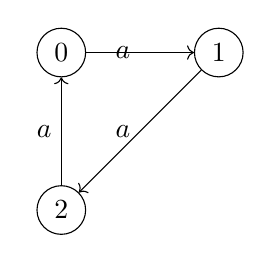
\begin{tikzpicture}
    % Place the nodes using relative positioning
    \node[shape=circle,draw=black] (0) at (0,2) {0};
    \node[shape=circle,draw=black] (1) at (2,2) {1};
    \node[shape=circle,draw=black] (2) at (0,0) {2};

    \path [->](0) edge node[left] {$a$} (1);
    \path [->](1) edge node[left] {$a$} (2);
    \path [->](2) edge node[left] {$a$} (0);
    
\end{tikzpicture}

\section*{Exercise 30}
The set of strings over \{\textit{a,b,c}\} in which the total number of \textit{a}'s is divisible by three.

\section*{Exercise 31}
The set of strings over \{\textit{a,b}\} in which every \textit{a} is either immediately preceded o immediately followed by \textit{b}, for example, \textit{baab}, \textit{aba}, and \textit{b}.

\section*{Exercise 32}
The set of strings of odd length over \{\textit{a,b}\} that contain the substring \textit{bb}.

\section*{Exercise 33}
The set of strings of even length over \{\textit{a,b,c}\} that contain exactly one \textit{a}.

\section*{Exercise 34}
The set of strings over \{\textit{a,b,c}\} with an odd number of occurrences of the substring \textit{ab}.

\section*{Exercise 35}
The set of strings of odd length over \{\textit{a,b}\} that contain exactly two \textit{b}'s.

\section*{Exercise 36}
The set of strings over \{\textit{a,b}\} with an even number of \textit{a}'s or an odd number of \textit{b}'s.

\end{document}
